\section{Approach overview}
\label{sec:approach}
%Compared to other code generation approaches, the philosophy of XSeparation is different.
This section presents the overview of our approach.
The latter consists of a mapping mechanism between architecture model and code, and a synchronization mechanism using the mapping as a means to synchronize the model and code.% to establish a bidirectional mapping between architecture model and code.

Fig. \ref{fig:mappingoverview} shows the overview of our approach.
The mapping mechanism is formed by a bidirectional mapping and a text-to-text transformation and described as belows.
%\subsection{Approach overview}
%The reason that makes the model-code synchronization hard is the lack of a bidirectional mapping between architecture and implementation.
%To establish a bidirectional mapping, we therefore raise the abstraction level of a standard programming language by introducing additional programming constructs.
%We demonstrate the case, in which the programming language is C++.
%Fig. \ref{fig:mappingoverview} shows the overview of our approach.
%From a standard programming language (such as C++), the additional constructs are added to it. 
%We establish a bidirectional mapping between the architecture model and the \tb{Extended code} to which the programmers make modifications.



\begin{figure}
	\centering
	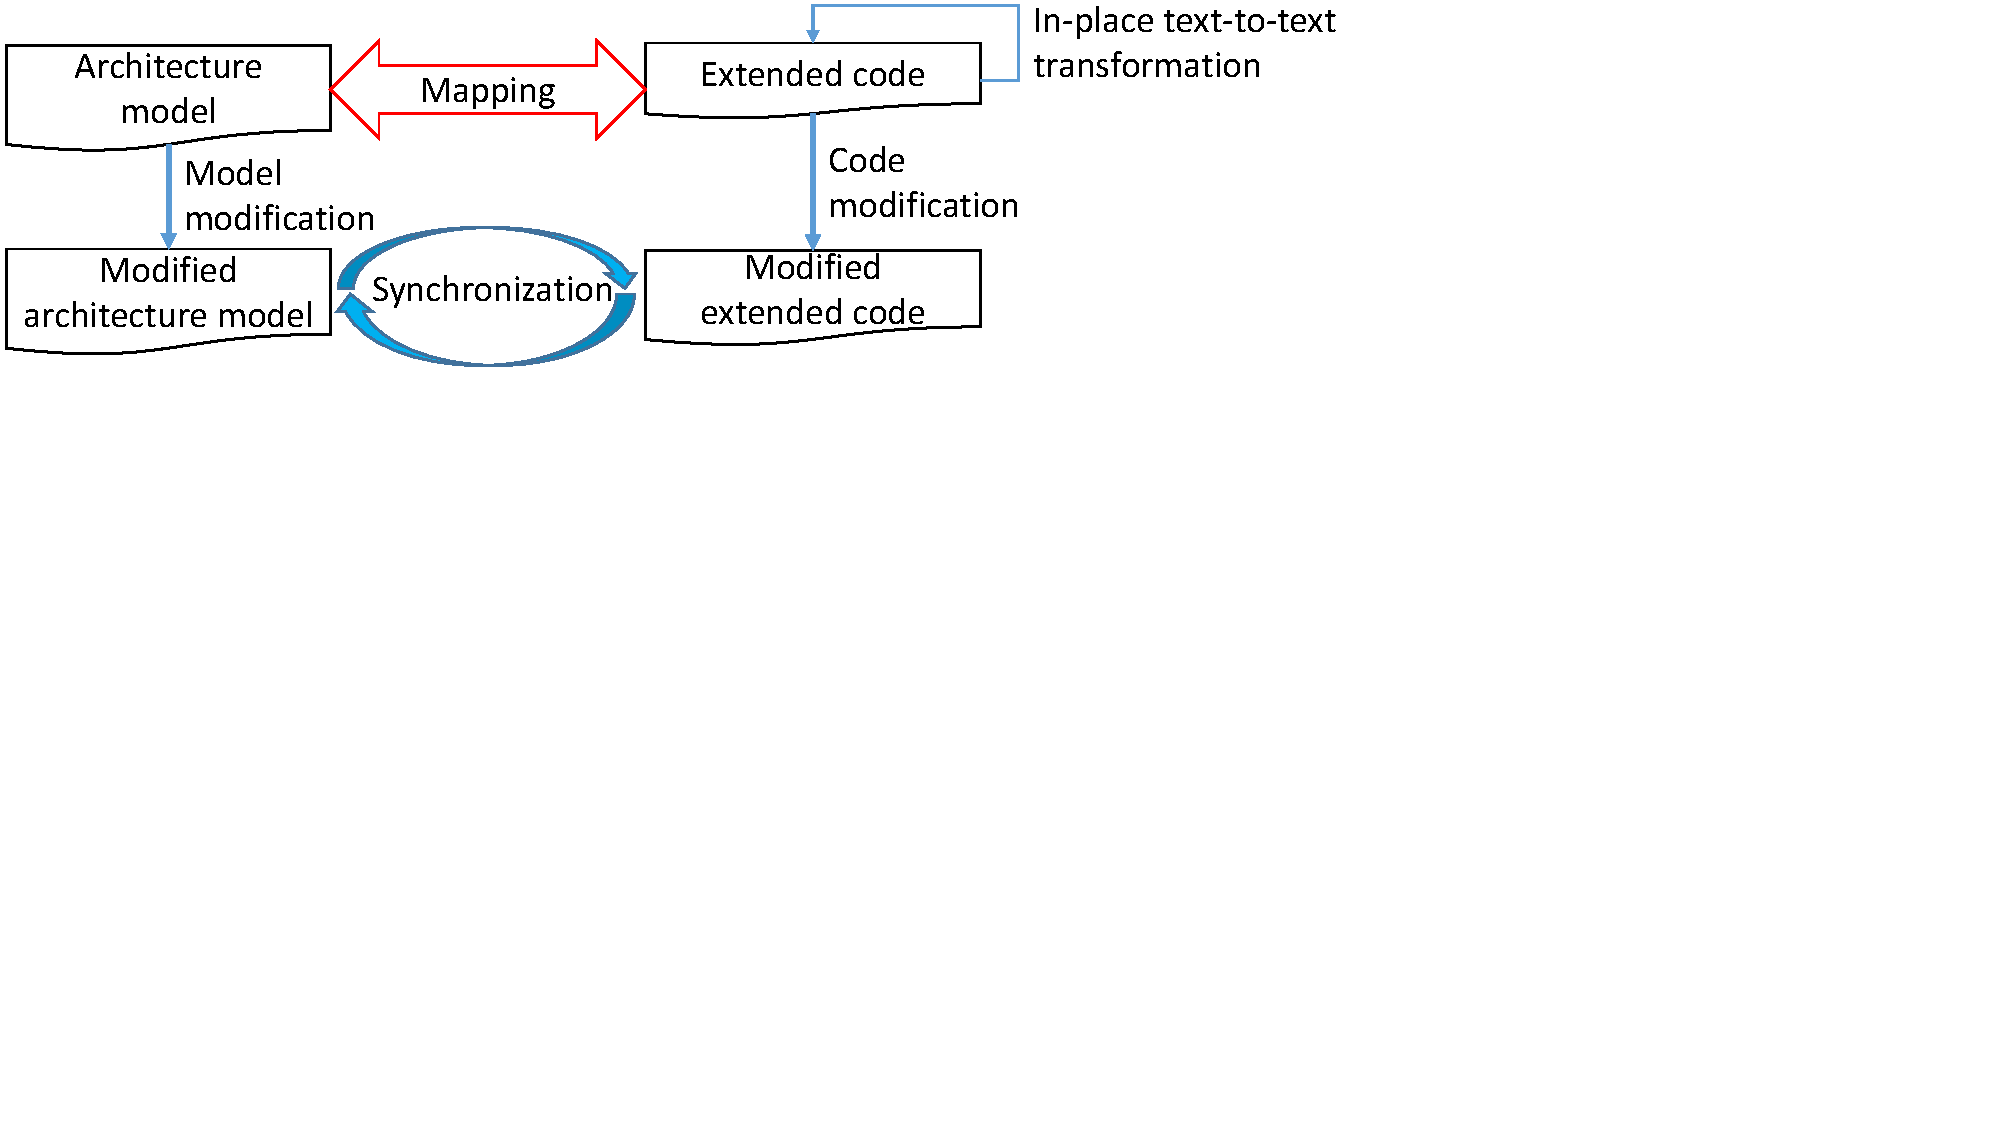
\includegraphics[clip, trim=0cm 12.5cm 9.6cm 0cm, width=\columnwidth]{figures/approachoverview.pdf}
	\caption{Approach overview} 
	\label{fig:mappingoverview}
\end{figure}

\noindent
\tb{Architecture model:}
The architecture designed by using the UML Class, Composite Structure, and State Machine concepts. 
The architecture model might be modified by the software architects or indirectly updated by propagating code modifications back to the model.

%\vspace{0.1cm}
\noindent
\tb{Mapping:}
The mapping consists of a set of correspondences \cite{Brambilla:2012:MSE:2432361} between elements of UML and the extended language (see the extended language and code). 
This mapping is bidirectional and is used as a means to ease the model-code synchronization.

%\vspace{0.1cm}
\noindent
\tb{Extended language and code:}
To build a bidirectional mapping between architecture model and code, we raise the abstraction level of a standard object-oriented programming language, whose language elements are at a lower level of abstraction than architecture elements \cite{DeSilva2012}. 
We tailor a standard object-oriented language by adding additional/ad-hoc programming constructs for the UML elements that have no direct representations in common programming languages, notable UML ports, connectors, and State Machine elements.
We choose these model elements because ports and connectors are widely proposed in many Architecture Description Languages (ADLs) \cite{Allen:1997:FBA:258077.258078}, and state machines are suitable to the modeling of the behavior of components in reactive systems.
The \ti{extended language} is the standard language with the additional constructs.
It is as close as possible to the existing standard language in order to be suitable for programmers perception to minimize additional learning efforts.
The \tb{Extended Code} conforms to the \ti{extended language}. 
%It is standard code but containing our added/ad-hoc programming constructs for modeling concepts that have no direct representation in common object-oriented languages, notably ports, connectors and state-machine elements.
%The reason of adding additional programming constructs to the standard programming language is to raise the abstraction level of a standard programming language, 
Programmers can therefore change the architecture model or the fine-grained code behavior at the code level while the code modifications can be reflected to the model by our synchronization mechanism. 
%to raise the abstraction level of a standard programming language by introducing additional programming constructs.
The additional constructs are created by using specialized mechanisms of the standard language such as templates, and macros in C++ or annotations in Java.
The \tb{Extended code} containing the additional constructs syntactically conforms to the standard programming language. 
By this way, the \tb{Extended code} can seamlessly reuse legacy code or library written in the standard programming language. 
This is especially important because current complex systems rely on a lot of library support \cite{Zhai:2016:AMG:2884781.2884881}.%and programming facilities such as syntax highlighting and auto-completion in Integrated Development Environments (IDEs) for assisting the development of the \tb{Extended code}. 
%\tb{Extended code} is translated into \tb{Standard code}. \tb{Extended code} and \tb{Extended code} are then combined to be executable.
%The latter is semantically closer to the architecture since it adds language constructs for modeling concepts that have no direct representation in common object-oriented languages, notably ports, connectors and state-machine elements. 

In the following sections, we use the terms \ti{Extended Code} and \ti{code} interchangeably and \ti{Extended language} refers to the standard language with our additional constructs.




%\vspace{0.1cm}
\noindent
\tb{In-place transformation:}
The additional programming constructs are used to ease the connections from code to architecture model.
However, they are natively not executable.
The in-place transformation utilizes the information in the extended code to complement the programming additional constructs so that these constructs are executable.

%\vspace{0.1cm}
\noindent
\tb{Model modification:}
Software architects make modifications/changes to the architecture design model during development.  

%\vspace{0.1cm}
\noindent
\tb{Code modification:}
Programmers make modifications/changes to the extended code during development.

%\vspace{0.1cm}
\noindent
\tb{Synchronization:}
Once the model and/or the code are/is modified, the synchronization reflects modifications made in one artifact to the other artifact and vice-versa.

In the following sections, we give the details of the mapping and synchronization.